%!TEX root = ../main.tex

\section{Experimental setup}
\label{sec:setup}

The experiment consists of several components. A schematic setup can be seen in 
\autoref{fig:setup}. The $\gamma$-source is moving at a velocity relative to the lab 
frame. The velocity can be adjusted via a digital function generator (DFG), 
Mössbauer velocity calibrator (MVC), Mössbauer velocity transducer (MVT), and 
Mössbauer driving unit (MDU). An absorber can be placed in the beam path of the 
high-energy photons. Based on their energy, resonant absorption occurs and the $\gamma$'s are either transmitted or 
absorbed by the target. The number of transmitted photons is counted by a 1024 
channel multi-channel-scaler (MCS). The various other components of the setup (VV, 
etc.) are used mainly for data acquisition (DAQ) purposes, more detailed information 
on the individual building blocks can be taken from \cite{Sch17}.

\begin{figure}[h]
	\centering
	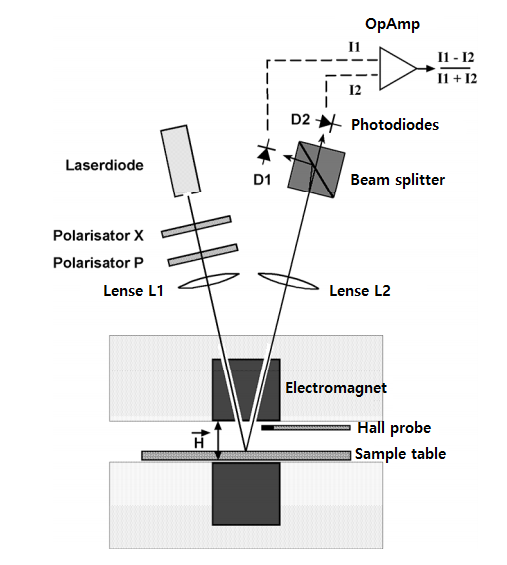
\includegraphics[width=0.8\textwidth]{./fig/setup.png}
	\caption{A schematic overview of the experiment components. The Mössbauer 
	driving unit (MDU) moves the $\gamma$-source at a velocity relative to the 
	multi-channel-scaler (MCS). The exact velocity can be controlled via a 
	digital function generator (DFG), Mössbauer velocity transducer (MVT) and is 
	monitored by an interferometer.}
	\label{fig:setup}
\end{figure}
